\section{Building and Training a Simple RNN Model using PyTorch for
Predicting Sine Wave
Patterns}\label{building-and-training-a-simple-rnn-model-using-pytorch-for-predicting-sine-wave-patterns}

\begin{lstlisting}[language=Python]
import torch
import torch.nn as nn
import torch.optim as optim
import numpy as np
import matplotlib.pyplot as plt
\end{lstlisting}

\subsubsection{Generate data}\label{generate-data}

Let's create a simple dataset to train our network on. We'll use a sine
wave as the input sequence and try to predict the next value in the
sequence. We'll create a dataset of 1000 sequences with 10 time steps
each.

\begin{lstlisting}[language=Python]
timesteps = 10
data_size = 1000

input_data = np.zeros((data_size, timesteps, 1))
output_data = np.zeros((data_size, 1))

for i in range(data_size):
    rand_offset = np.random.random() * 2 * np.pi
    input_data[i, :, 0] = np.sin(np.linspace(0.0 + rand_offset, 3 * np.pi + rand_offset, num=timesteps))
    output_data[i, 0] = np.sin(3 * np.pi + rand_offset)
\end{lstlisting}

\textbf{Explanation}

First, we define two variables: \lstinline{timesteps} and
\lstinline{data_size}.
\lstinline{timesteps} determines the length of each input sequence, and \lstinline{data_size} determines the number of samples we want to generate.\newline

Next, we create two NumPy arrays to hold our input and output data.
\lstinline{input_data} is a 3-dimensional array with
shape \lstinline{(data_size, timesteps, 1)}. This means
that we have \lstinline{data_size} samples, each with
\lstinline{timesteps} time steps, and 1 feature at each
time step. \lstinline{output_data} is a 2-dimensional
array with shape \lstinline{(data_size, 1)}, which means
that we have \lstinline{data_size} output samples, each
with 1 feature. \newline

Then, we loop through each sample in our dataset using a for loop. For
each sample, we generate a random offset between \(0\) and \(2 \pi\) using
\lstinline{np.random.random() * 2 * np.pi}. This offset is
used to shift the sine wave we generate for the input sequence. \newline

We generate the input sequence by calling
\lstinline{np.linspace} to create a sequence of timesteps
values evenly spaced between \(0\) and \(3 \pi\) (inclusive), and adding the random
offset to each value. We then pass this sequence through the
\lstinline{np.sin} function to generate the sine wave. \newline

We generate the output value by computing the sine of \(3 \pi\) plus the random
offset. This is the next value in the sine wave after the input sequence
ends. \newline

Finally, we assign the input sequence and output value to the
corresponding rows in \lstinline{input_data} and
\lstinline{output_data}, respectively. \newline

Overall, this code generates a dataset of
\lstinline{data_size} samples, where each sample consists
of an input sequence of \lstinline{timesteps} time steps
and an output value that is the next value in the sine wave after the
input sequence ends. The offset applied to each sample's sine wave
introduces variability to the dataset, making it more challenging for
our model to learn the underlying pattern in the data. \newline

Let's visualize this data.

\begin{lstlisting}[language=Python]
fig, axs = plt.subplots(2, 3, figsize=(12, 8))

for i in range(2):
    for j in range(3):
        # plot input sequence
        axs[i,j].plot(input_data[i+j,:,0], label='Input')

        # plot output value with big marker
        axs[i,j].plot(range(timesteps-1, timesteps), output_data[i+j], marker='o', markersize=10, label='Output')

        # set plot title, axis labels, and legend
        axs[i,j].set_title(f'Sample {i+j+1}')
        axs[i,j].set_xlabel('Time Step')
        axs[i,j].set_ylabel('Feature Value / Value')
        axs[i,j].legend()

plt.suptitle('Input and Output Sequences')
plt.tight_layout()
plt.show()
\end{lstlisting}

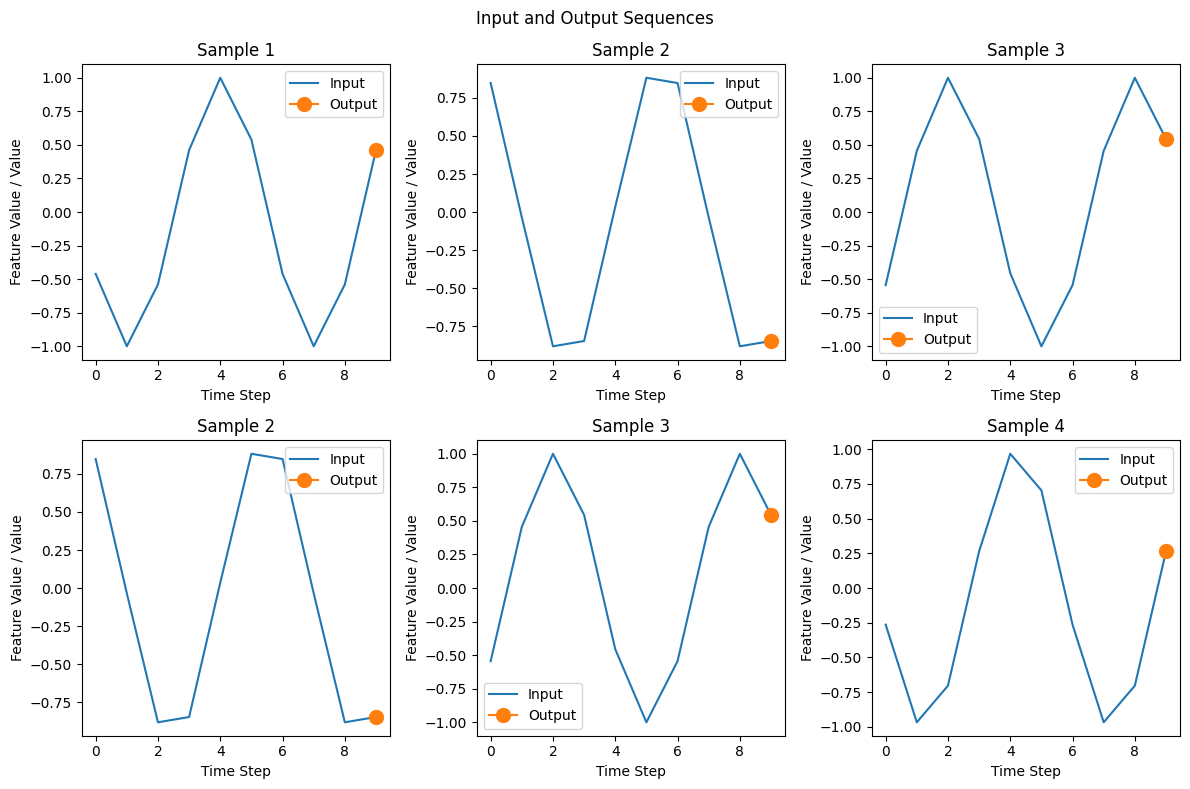
\includegraphics{img//rnn//intro/output_5_0.png}

Now, let's split the dataset into training and testing sets:

\begin{lstlisting}[language=Python]
train_size = int(data_size * 0.8)

X_train = input_data[:train_size, :, :]
y_train = output_data[:train_size, :]

X_test = input_data[train_size:, :, :]
y_test = output_data[train_size:, :]
\end{lstlisting}

\subsubsection{Define the RNN model}\label{define-the-rnn-model}

We'll use a simple RNN with a single hidden layer:

\begin{lstlisting}[language=Python]
class Net(nn.Module):
    def __init__(self):
        super(Net, self).__init__()

        # Create a new RNN layer with 1 input feature, 32 hidden units, and 1 layer
        self.rnn = nn.RNN(input_size=1, hidden_size=32, num_layers=1, batch_first=True)

        # Create a new fully connected layer with 32 input features and 1 output feature
        self.fc = nn.Linear(32, 1)

    def forward(self, x):
        """
        Passes the input tensor through the RNN and the fully connected layer.

        Args:
            x (torch.Tensor): Input tensor of shape (batch_size, sequence_length, input_size)

        Returns:
            torch.Tensor: Output tensor of shape (batch_size, 1)
        """
        # Pass the input tensor through the RNN layer, which returns a new tensor with
        # shape (batch_size, sequence_length, hidden_size)
        rnn_out, _ = self.rnn(x)

        # Pass the last output from the RNN layer through the fully connected layer,
        # which returns a new tensor with shape (batch_size, 1)
        fc_out = self.fc(rnn_out[:, -1, :])

        # Return the output tensor
        return fc_out
\end{lstlisting}

\textbf{Explanation}:

The Net class inherits from the PyTorch nn.Module class, which allows us
to define our neural network as a collection of layers that can be
trained together. \newline

In the \lstinline{__init__} method, we define our RNN
layer and fully connected layer:

\begin{itemize}
\item
  \lstinline{self.rnn:} A new
  \lstinline{nn.RNN} layer with 1 input feature
  (\lstinline{input_size=1}), 32 hidden units
  (\lstinline{hidden_size=32}), and 1 layer
  (\lstinline{num_layers=1}). We
  set\lstinline{batch_first=True} so that the input
  tensor has shape
  \lstinline{(batch_size, sequence_length, input_size)}.
\item
  \lstinline{self.fc}: A new
  \lstinline{nn.Linear} layer with 32 input features
  (\lstinline{in_features=32}) and 1 output feature
  (\lstinline{out_features=1}).
\end{itemize}

In the forward method, we define how the input tensor is passed through
our network:

\begin{itemize}
\item
  We pass the input tensor \lstinline{x} through the RNN layer using \lstinline{self.rnn(x)}. This returns a new tensor with shape \lstinline{(batch_size, sequence_length, hidden_size)}.
\item
  We take the last output from the RNN layer using
  \lstinline{rnn_out[:, -1, :]}. This returns a tensor
  with shape \lstinline{(batch_size, hidden_size)}.
\item
  We pass this last output through the fully connected layer using
  \lstinline{self.fc(rnn_out[:, -1, :])}. This returns a
  tensor with shape \lstinline{(batch_size, 1)}.
\item
  We return the output tensor.
\end{itemize}

Note that the \lstinline{_} in
\lstinline{rnn_out, _ = self.rnn(x)} indicates that we
are only interested in the first output of
\lstinline{self.rnn(x)}, which is the output tensor, and
not the second output, which is the final hidden state of the RNN layer.
Since we are not using this hidden state, we can ignore it by assigning
it to \lstinline{_}.

\begin{lstlisting}[language=Python]
net = Net()
\end{lstlisting}

We'll use mean squared error loss and the Adam optimizer:

\begin{lstlisting}[language=Python]
criterion = nn.MSELoss()
optimizer = optim.Adam(net.parameters(), lr=0.01)
\end{lstlisting}

\textbf{Explanation}

The MSE loss function is a commonly used loss function for regression
problems. It measures the average of the squared differences between the
predicted output and the true output. In our case, we want our RNN to
predict the sine wave value at the last time step given the input
sequence, which is a regression problem. Therefore, using the MSE loss
function is appropriate. \newline

The Adam optimizer is a popular stochastic gradient descent optimizer
that is known for its efficiency and robustness. It adapts the learning
rate for each parameter based on the first and second moments of the
gradients. In other words, it adjusts the learning rate for each weight
in the network based on how much and how quickly the weight is changing.
This helps the optimizer converge faster and more reliably than other
stochastic gradient descent optimizers. Therefore, using the Adam
optimizer is a good choice for training our RNN. \newline

In summary, we used the MSE loss function because we have a regression
problem, and we used the Adam optimizer because it is efficient and
robust. \newline

Now, we'll define our training loop. We'll train the network for 70
epochs and calculate the training and validation loss after each epoch:

\begin{lstlisting}[language=Python]
train_losses = []
val_losses = []

for epoch in range(70):
    net.train()
    optimizer.zero_grad()

    outputs = net(torch.Tensor(X_train))
    loss = criterion(outputs, torch.Tensor(y_train))

    loss.backward()
    optimizer.step()

    train_losses.append(loss.item())

    net.eval()
    with torch.no_grad():
        outputs = net(torch.Tensor(X_test))
        val_loss = criterion(outputs, torch.Tensor(y_test))
        val_losses.append(val_loss.item())

    print('Epoch [{}/{}], Train Loss: {:.4f}, Val Loss: {:.4f}'
          .format(epoch+1, 70, loss.item(), val_loss.item()))
\end{lstlisting}

\begin{lstlisting}
Epoch [1/70], Train Loss: 0.5126, Val Loss: 0.3841
Epoch [2/70], Train Loss: 0.3981, Val Loss: 0.2881
Epoch [3/70], Train Loss: 0.2992, Val Loss: 0.1705
Epoch [4/70], Train Loss: 0.1772, Val Loss: 0.0410
Epoch [5/70], Train Loss: 0.0424, Val Loss: 0.0199
Epoch [6/70], Train Loss: 0.0204, Val Loss: 0.0971
Epoch [7/70], Train Loss: 0.1003, Val Loss: 0.0628
Epoch [8/70], Train Loss: 0.0647, Val Loss: 0.0096
Epoch [9/70], Train Loss: 0.0099, Val Loss: 0.0073
Epoch [10/70], Train Loss: 0.0075, Val Loss: 0.0299
Epoch [11/70], Train Loss: 0.0306, Val Loss: 0.0419
Epoch [12/70], Train Loss: 0.0432, Val Loss: 0.0386
Epoch [13/70], Train Loss: 0.0400, Val Loss: 0.0251
Epoch [14/70], Train Loss: 0.0260, Val Loss: 0.0093
Epoch [15/70], Train Loss: 0.0097, Val Loss: 0.0011
Epoch [16/70], Train Loss: 0.0011, Val Loss: 0.0050
Epoch [17/70], Train Loss: 0.0050, Val Loss: 0.0139
Epoch [18/70], Train Loss: 0.0143, Val Loss: 0.0169
Epoch [19/70], Train Loss: 0.0174, Val Loss: 0.0120
Epoch [20/70], Train Loss: 0.0124, Val Loss: 0.0051
Epoch [21/70], Train Loss: 0.0053, Val Loss: 0.0019
Epoch [22/70], Train Loss: 0.0020, Val Loss: 0.0032
Epoch [23/70], Train Loss: 0.0034, Val Loss: 0.0062
Epoch [24/70], Train Loss: 0.0064, Val Loss: 0.0080
Epoch [25/70], Train Loss: 0.0082, Val Loss: 0.0075
Epoch [26/70], Train Loss: 0.0077, Val Loss: 0.0053
Epoch [27/70], Train Loss: 0.0055, Val Loss: 0.0029
Epoch [28/70], Train Loss: 0.0030, Val Loss: 0.0017
Epoch [29/70], Train Loss: 0.0016, Val Loss: 0.0021
Epoch [30/70], Train Loss: 0.0020, Val Loss: 0.0031
Epoch [31/70], Train Loss: 0.0031, Val Loss: 0.0035
Epoch [32/70], Train Loss: 0.0037, Val Loss: 0.0032
Epoch [33/70], Train Loss: 0.0034, Val Loss: 0.0025
Epoch [34/70], Train Loss: 0.0026, Val Loss: 0.0016
Epoch [35/70], Train Loss: 0.0017, Val Loss: 0.0010
Epoch [36/70], Train Loss: 0.0010, Val Loss: 0.0009
Epoch [37/70], Train Loss: 0.0010, Val Loss: 0.0013
Epoch [38/70], Train Loss: 0.0013, Val Loss: 0.0017
Epoch [39/70], Train Loss: 0.0017, Val Loss: 0.0018
Epoch [40/70], Train Loss: 0.0018, Val Loss: 0.0014
Epoch [41/70], Train Loss: 0.0014, Val Loss: 0.0008
Epoch [42/70], Train Loss: 0.0008, Val Loss: 0.0004
Epoch [43/70], Train Loss: 0.0004, Val Loss: 0.0004
Epoch [44/70], Train Loss: 0.0004, Val Loss: 0.0006
Epoch [45/70], Train Loss: 0.0007, Val Loss: 0.0009
Epoch [46/70], Train Loss: 0.0010, Val Loss: 0.0009
Epoch [47/70], Train Loss: 0.0010, Val Loss: 0.0006
Epoch [48/70], Train Loss: 0.0007, Val Loss: 0.0003
Epoch [49/70], Train Loss: 0.0003, Val Loss: 0.0001
Epoch [50/70], Train Loss: 0.0001, Val Loss: 0.0002
Epoch [51/70], Train Loss: 0.0002, Val Loss: 0.0005
Epoch [52/70], Train Loss: 0.0004, Val Loss: 0.0006
Epoch [53/70], Train Loss: 0.0006, Val Loss: 0.0005
Epoch [54/70], Train Loss: 0.0005, Val Loss: 0.0002
Epoch [55/70], Train Loss: 0.0002, Val Loss: 0.0001
Epoch [56/70], Train Loss: 0.0001, Val Loss: 0.0001
Epoch [57/70], Train Loss: 0.0001, Val Loss: 0.0002
Epoch [58/70], Train Loss: 0.0002, Val Loss: 0.0003
Epoch [59/70], Train Loss: 0.0003, Val Loss: 0.0003
Epoch [60/70], Train Loss: 0.0003, Val Loss: 0.0002
Epoch [61/70], Train Loss: 0.0002, Val Loss: 0.0001
Epoch [62/70], Train Loss: 0.0001, Val Loss: 0.0000
Epoch [63/70], Train Loss: 0.0000, Val Loss: 0.0001
Epoch [64/70], Train Loss: 0.0001, Val Loss: 0.0001
Epoch [65/70], Train Loss: 0.0001, Val Loss: 0.0002
Epoch [66/70], Train Loss: 0.0002, Val Loss: 0.0001
Epoch [67/70], Train Loss: 0.0001, Val Loss: 0.0000
Epoch [68/70], Train Loss: 0.0000, Val Loss: 0.0000
Epoch [69/70], Train Loss: 0.0000, Val Loss: 0.0000
Epoch [70/70], Train Loss: 0.0000, Val Loss: 0.0001
\end{lstlisting}

\textbf{Explanation}

\begin{itemize}
\item
  \lstinline{train_losses = []} and
  \lstinline{val_losses = []}: These create two empty
  lists to store the training and validation losses for each epoch.
\item
  \lstinline{for epoch in range(70)}: This starts a loop
  that will run for 70 epochs, during which the network will be trained
  and evaluated.
\item
  \lstinline{net.train()} sets the network in training
  mode.
\item
  \lstinline{optimizer.zero_grad()} zeroes out the
  gradients of the network's parameters, so that they don't accumulate
  from one iteration to the next.
\item
  \lstinline{outputs = net(torch.Tensor(X_train))} passes
  the training input data \lstinline{X_train} through the
  network to get the predicted output \lstinline{outputs}.
\item
  \lstinline{loss = criterion(outputs, torch.Tensor(y_train))}
  calculates the training loss between the predicted output
  \lstinline{outputs} and the true output
  \lstinline{y_train} using the mean squared error (MSE)
  loss function.
\item
  \lstinline{loss.backward()} computes the gradients of
  the loss with respect to the network's parameters.
\item
  \lstinline{optimizer.step()} updates the network's
  parameters based on the computed gradients and the optimizer's update
  rule (in this case, Adam).
\item
  \lstinline{train_losses.append(loss.item())} appends
  the training loss for the current epoch to the
  \lstinline{train_losses} list.
\item
  \lstinline{net.eval()} sets the network in evaluation
  mode.
\item
  \lstinline{with torch.no_grad()}: temporarily disables
  gradient computation to save memory and speed up the evaluation
  process.
\item
  \lstinline{outputs = net(torch.Tensor(X_test))} passes
  the validation input data \lstinline{X_test} through
  the network to get the predicted output
  \lstinline{outputs}.
\item
  \lstinline{val_loss = criterion(outputs, torch.Tensor(y_test))}
  calculates the validation loss between the predicted output
  \lstinline{outputs} and the true output
  \lstinline{y_test} using the mean squared error (MSE)
  loss function.
\item
  \lstinline{val_losses.append(val_loss.item())} appends
  the validation loss for the current epoch to the
  \lstinline{val_losses} list.
\item
  \lstinline|print('Epoch [{}/{}], Train Loss: {:.4f}, Val Loss: {:.4f}'.format(epoch+1, 100, loss.item(), val_loss.item()))|
  prints the current epoch number, the training loss, and the validation
  loss.
\end{itemize}

The training loop trains the RNN on the training data for 70 epochs
using the Adam optimizer and the mean squared error loss function. The
loop also computes and records the training and validation losses for
each epoch, so that the performance of the model can be analyzed over
time.\newline

Finally, let's plot the training and validation loss over epochs:

\begin{lstlisting}[language=Python]
plt.plot(train_losses, label='Train Loss')
plt.plot(val_losses, label='Validation Loss')
plt.legend()
plt.show()
\end{lstlisting}

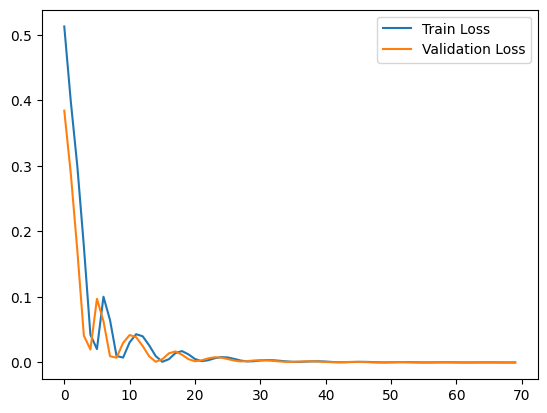
\includegraphics{img//rnn//intro/output_19_0.png}

And that's it! We've successfully trained a simple RNN to predict the
next value in a sine wave sequence.
